
In the architecture design of the front-end,  
the goal is to meet the user's usage requirements, 
which includes intuitive operations for data manipulation (create, read, update, delete) 
and simple creation of data channels,as well as managing and visualizing data channels.

Therefore, the front-end utilizes the React framework based on view design 
and the Redux framework based on state and data flow.

The structure of the React framework divides the web page into multiple components 
based on modularity. Each component has its own state and properties.
Components are categorized into container components, presentational components, 
and functional components. 

Container components manage data and state, presentational components display data 
and state, and functional components implement specific functionalities.

In this project, following the structure of the React framework and adopting a component-based approach,
the entire project is divided into the following components:

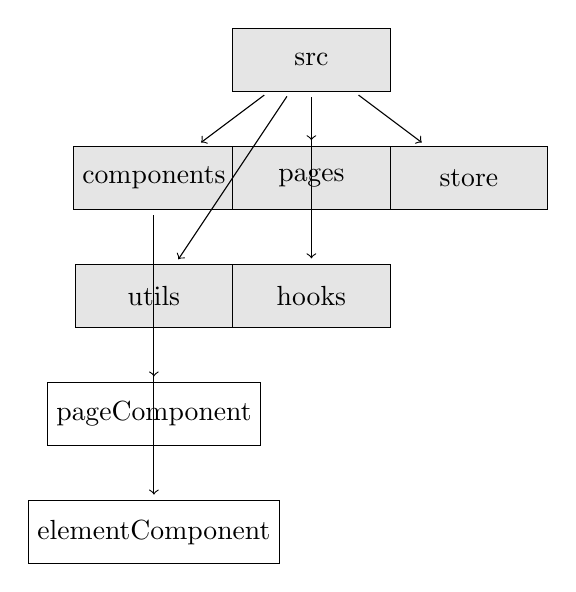
\begin{tikzpicture}[
    file/.style={draw, rectangle, minimum width=2cm, minimum height=0.8cm},
    folder/.style={draw, rectangle, minimum width=2cm, minimum height=0.8cm, fill=gray!20},
    arrow/.style={->, shorten >=2pt, shorten <=2pt}
]

% Folders
\node[folder] (src) at (0,0) {src};
\node[folder] (components) at (-2,-1.5) {components};
\node[folder] (pages) at (0,-1.5) {pages};
\node[folder] (store) at (2,-1.5) {store};
\node[folder] (utils) at (-2,-3) {utils};
\node[folder] (hooks) at (0,-3) {hooks};

% Files
\node[file] (pageComponent) at (-2,-4.5) {pageComponent};
\node[file] (elementComponent) at (-2,-6) {elementComponent};
% ... add more files

% Connections
\draw[arrow] (src) -- (components);
\draw[arrow] (src) -- (pages);
\draw[arrow] (src) -- (store);
\draw[arrow] (src) -- (utils);
\draw[arrow] (src) -- (hooks);
\draw[arrow] (components) -- (pageComponent);
\draw[arrow] (components) -- (elementComponent);
% ... add more connections

\end{tikzpicture}


